
% \titlegraphic{\hfill\includegraphics[height=1.5cm]{logo.pdf}}

\documentclass[xcolor=pdftex,dvipsnames,table,numbers,hyperref={pdfpagelabels=false},compress]{beamer}
%\usepackage{requiredPackage}
\usepackage{amsmath}
\usepackage{graphicx}
\usepackage{amsfonts}
\usepackage{amssymb}

\usepackage{tabularx}
\usepackage{epstopdf}
\usepackage{overpic}
\usepackage{url}
\usepackage{calrsfs}
\usepackage{mathrsfs}
\usepackage{epsfig}
\usepackage{cancel}
\usepackage{changepage}

\usepackage{tikz}
\usepackage[customcolors]{hf-tikz} 

\usepackage{lmodern}
%\usepackage{mystyle}
\usepackage{subfig}
\usepackage{pifont}
\usepackage{tabu}
\usepackage{xcolor}
\usepackage{algorithm}
\usepackage{algpseudocode}
%\usepackage{enumitem}
\usepackage{remreset}
\usepackage{etoolbox}
\usepackage{comment} % end and begin comment
%\usepackage{dtklogos} 
\usepackage{listings}
\lstset{breaklines=true} 

\newcommand{\gline}{\textcolor{gray}{\hline}}
\newcommand{\cmark}{\ding{51}}%
\newcommand{\xmark}{\ding{55}}%
\newcommand{\gcheck}{\textcolor{blue}{\Large \cmark}}
\newcommand{\rcross}{\textcolor{red}{\Large \xmark}}
\newcommand{\tkt}{\tilde{K}_\theta}
\newcommand{\kt}{K_\theta}
\newcommand{\ind}{\overset{ind}{\sim}}
\newcommand{\plim}{\overset{p}{\rightarrow}}
\newcommand{\cx}{\frac {X'X}n}
\newcommand{\cz}{\frac {Z'Z}n}
\newcommand{\ccz}{\frac {Z'Z}n - \Sigma_A}
\newcommand{\czy}{\frac {Z'y}n}
\newcommand{\cyz}{\frac {y'Z}n}
\newcommand{\cxy}{\frac {X'y}n}
\newcommand{\cyx}{\frac {y'X}n}
\newcommand{\myitem}{\vskip3mm \item}

\newcommand{\calS}{{\cal S}}
\newcommand{\calA}{{\cal A}}
\newcommand{\calK}{{\cal K}}
\newcommand{\calX}{{\cal X}}
\newcommand{\calD}{{\cal D}}
\newcommand{\calG}{{\cal G}}
\newcommand{\calT}{{\cal T}}
\newcommand{\calU}{{\cal U}}
\newcommand{\calR}{{\cal R}}
\newcommand{\tp}{\tilde{p}}
\newcommand{\tildebC}{\tilde{\bC}}
\newcommand{\calL}{{\cal L}}

\newcommand{\blam}{ \mbox{\boldmath $ \lambda $} }
\newcommand{\bet}{ \mbox{\boldmath $ \eta $} }
\newcommand{\bome}{ \mbox{\boldmath $ \omega $} }
\newcommand{\bbet}{ \mbox{\boldmath $ \beta $} }
\newcommand{\bbeta}{ \mbox{\boldmath $ \beta $} }
\newcommand{\balph}{ \mbox{\boldmath $ \alpha $} }
\newcommand{\balpha}{ \mbox{\boldmath $ \alpha $} }
\newcommand{\bphi}{ \mbox{\boldmath $\phi$}}
\newcommand{\bzeta}{ \mbox{\boldmath $\zeta$}}
\newcommand{\bkap}{ \mbox{\boldmath $\kappa$}}
\newcommand{\bkappa}{ \mbox{\boldmath $\kappa$}}
\newcommand{\beps}{ \mbox{\boldmath $\epsilon$}}
\newcommand{\bepsilon}{ \mbox{\boldmath $\epsilon$}}
\newcommand{\bthet}{ \mbox{\boldmath $ \theta $} }
\newcommand{\btheta}{ \mbox{\boldmath $ \theta $} }
\newcommand{\blambda}{ \mbox{\boldmath $ \lambda $} }
\newcommand{\bnu}{ \mbox{\boldmath $\nu$} }
\newcommand{\bmu}{ \mbox{\boldmath $\mu$} }
\newcommand{\bGam}{ \mbox{\boldmath $\Gamma$} }
\newcommand{\bSig}{ \mbox{\boldmath $\Sigma$} }
\newcommand{\bSigma}{ \mbox{\boldmath $\Sigma$} }
\newcommand{\bPhi}{ \mbox{\boldmath $\Phi$} }
\newcommand{\bThet}{ \mbox{\boldmath $\Theta$} }
\newcommand{\bTheta}{ \mbox{\boldmath $\Theta$} }
\newcommand{\bDel}{ \mbox{\boldmath $\Delta$} }
\newcommand{\bDelta}{ \mbox{\boldmath $\Delta$} }
\newcommand{\bnabla}{ \mbox{\boldmath $\nabla$} }
\newcommand{\bLam}{ \mbox{\boldmath $\Lambda$} }
\newcommand{\bLambda}{ \mbox{\boldmath $\Lambda$} }
\newcommand{\bgam}{ \mbox{\boldmath $\gamma$} }
\newcommand{\bgamma}{ \mbox{\boldmath $\gamma$} }
\newcommand{\brho}{ \mbox{\boldmath $\rho$} }
\newcommand{\bdel}{ \mbox{\boldmath $\delta$} }
\newcommand{\bdelta}{ \mbox{\boldmath $\delta$} }
\newcommand{\sis}{\sigma^2}
\newcommand{\bOmega}{\mbox{\boldmath $\Omega$} }
\newcommand{\bPsi}{ {\boldsymbol \Psi} }
\newcommand{\btkt}{\boldsymbol{\tilde{K}}_\theta}
\newcommand{\pg}{P{\'o}lya-Gamma }

\newcommand{\bzero}{\textbf{0}}
\newcommand{\bones}{\textbf{1}}
\newcommand{\ba}{\textbf{a}}
\newcommand{\bb}{\textbf{b}}
\newcommand{\bB}{\textbf{B}}
%\newcommand{\bA}{\textbf{A}}
\newcommand{\bc}{\textbf{c}}
\newcommand{\bC}{\textbf{C}}
\newcommand{\bA}{\textbf{A}}
\newcommand{\bd}{\textbf{d}}
\newcommand{\bD}{\textbf{D}}
\newcommand{\be}{\textbf{e}}
\newcommand{\bE}{\textbf{E}}
\newcommand{\bk}{\textbf{k}}
\newcommand{\bK}{\textbf{K}}
\newcommand{\bh}{\textbf{h}}
\newcommand{\bs}{\textbf{s}}
\newcommand{\bS}{\textbf{S}}
\newcommand{\bH}{\textbf{H}}
\newcommand{\bI}{\textbf{I}}
\newcommand{\bt}{\textbf{t}}
\newcommand{\bu}{\textbf{u}}
\newcommand{\bv}{\textbf{v}}
\newcommand{\bw}{\textbf{w}}
\newcommand{\bW}{\textbf{W}}
\newcommand{\bx}{\textbf{x}}
\newcommand{\bX}{\textbf{X}}
\newcommand{\by}{\textbf{y}}
\newcommand{\bY}{\textbf{Y}}
\newcommand{\bz}{\textbf{z}}
\newcommand{\bZ}{\textbf{Z}}
\newcommand{\bL}{\textbf{L}}
\newcommand{\br}{\textbf{r}}
\newcommand{\bR}{\textbf{R}}
\newcommand{\bm}{\textbf{m}}
\newcommand{\bM}{\textbf{M}}
\newcommand{\given}{\,|\,}
\newcommand{\T}{\top}
\newcommand{\bV}{\textbf{V}}
\newcommand{\bJ}{\textbf{J}}
\newcommand{\blue}[1]{{\color{RoyalBlue!90} #1}}
\newcommand{\red}[1]{{\color{Red} #1}}
\newcommand{\green}[1]{{\color{Green} #1}}
\newcommand{\orange}[1]{{\color{Orange} #1}}
\newcommand{\titl}[1]{{\begin{large}\begin{center}#1\end{center}\end{large}}}

\newcommand{\tildea}{\tilde{a}}
\newcommand{\tildeba}{\tilde{\ba}}
\newcommand{\tildebv}{\tilde{\bv}}
\newcommand{\tildev}{\tilde{v}}
\newcommand{\tildeA}{\tilde{A}}
\newcommand{\tildeC}{\tilde{C}}
\newcommand{\tildeK}{\tilde{K}}
\newcommand{\tildew}{\tilde{w}}
\newcommand{\tildeu}{\tilde{u}}
\newcommand{\tildebw}{\tilde{\bw}}
\newcommand{\tildeeps}{\tilde{\epsilon}}
\newcommand{\tildebeps}{\tilde{\bepsilon}}
\newcommand{\eps}{\epsilon}
\newcommand{\sigs}{\sigma^2}
\newcommand{\taus}{\tau^2}
\newcommand{\iid}{\stackrel{\mathrm{iid}}{\sim}}

%\newcommand{\calS}{{\cal S}}
\newcommand{\calC}{{\cal C}}

%\documentclass[10pt]{beamer}

\usetheme{metropolis}
\usepackage{appendixnumberbeamer}

\usepackage{booktabs}
\usepackage[scale=2]{ccicons}

\usepackage{pgfplots}
\usepgfplotslibrary{dateplot}

\usepackage{xspace}
\newcommand{\themename}{\textbf{\textsc{metropolis}}\xspace}

\makeatletter
\@addtoreset{subfigure}{framenumber}% subfigure counter resets every frame
\makeatother

\makeatletter
\@addtoreset{figure}{framenumber}% subfigure counter resets every frame
\makeatother

\setbeamertemplate{caption}{\raggedright\insertcaption\par}
\captionsetup[subfigure]{labelformat=empty}


\title[]{Dynamic NNGP for Large Spatio-temporal Data}
\author{Andrew Finley$^1$ \& Jeffrey Doser$^2$}
	
\institute{
\begin{tiny}$^1$Department of Forestry, Michigan State University.\\
$^2$Department of Integrative Biology, Michigan State University.\end{tiny}
}

\date{May 15, 2023}


\begin{document}

\maketitle

\begin{frame}{Spatio-temporal Data}
	\begin{itemize}
		\item Data from \blue{multiple timepoints} at some or each of the locations
		\item Example: Climate data, air pollution data, house prices data
		\item Time points can be regular (hourly, daily, weekly) or irregular 
	\end{itemize}
	\vskip-9mm\begin{figure}[]
		\begin{center}
			{\subfloat[]{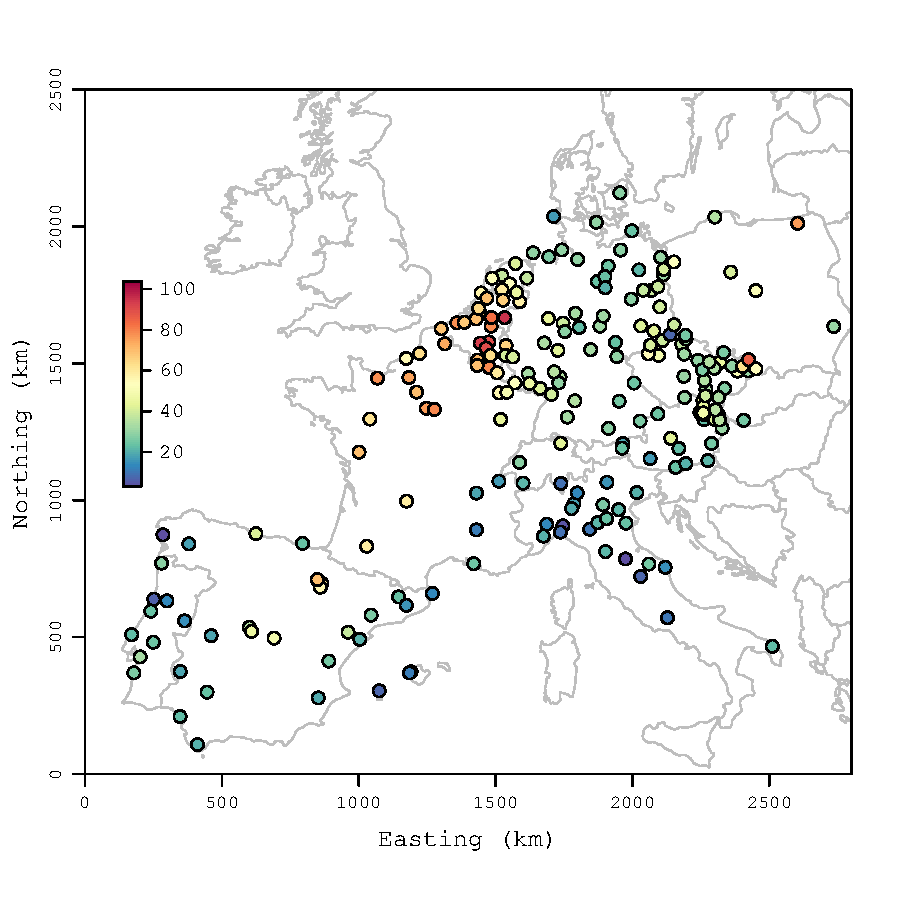
\includegraphics[width=5cm]{../figures/march-obs.pdf}}}
			\subfloat[]{{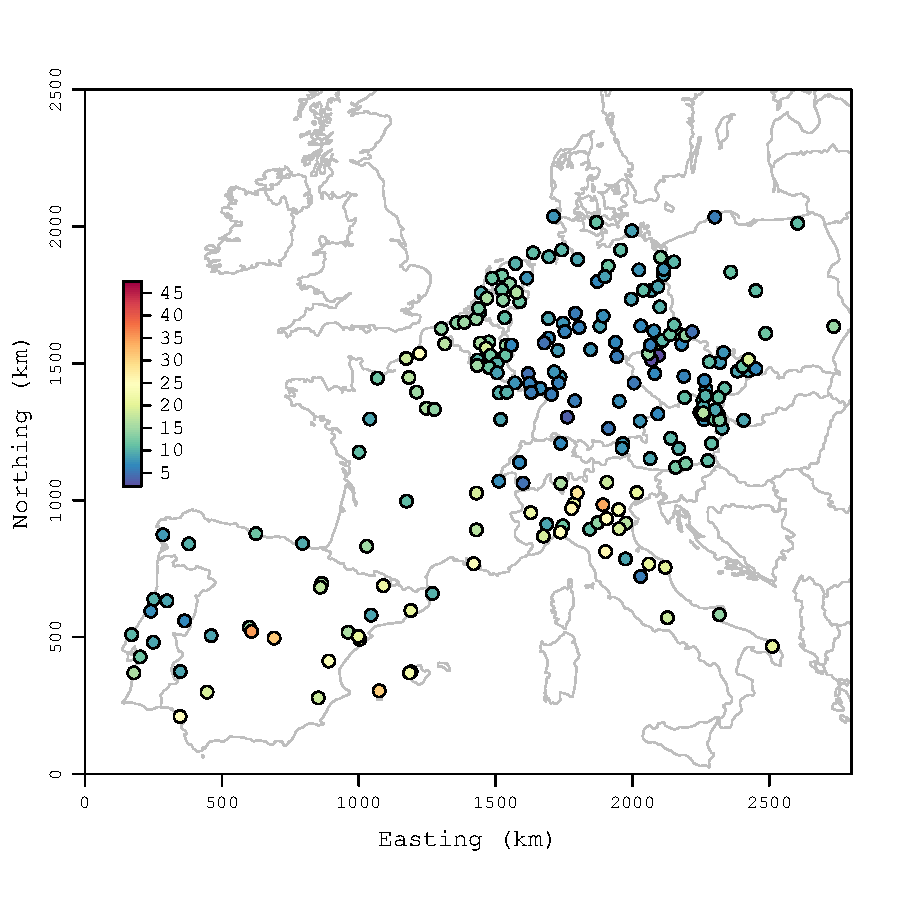
\includegraphics[width=5cm]{../figures/june-obs.pdf}}}
		\end{center}
	\vskip -8mm \caption{PM$_{10}$ levels in Europe in March, 2009 (left) and June, 2009 (right)}
	\end{figure}
\end{frame}

\begin{frame}{Discrete Time Continuous Space Models}

\begin{itemize}  
\myitem $y(s,t) = \underbrace{x_t'(s)\beta_t}_{\mbox{mean}} \qquad + \underbrace{u_t(s)}_{\mbox{{random effect}}} + \underbrace{\eps_s(t)}_{\mbox{iid  noise}}$
\myitem $\beta_t =\beta_{t-1}+\eta_t$, $\eta_t \sim N(0,\Sigma_t)$
\myitem $u_t(s) = u_{t-1}(s)+w_t(s)$
\myitem $w_t = (w_t(s_1),\ldots,w_t(s_K))' \ind N(0,C_S(\theta_t))$
\pause
\myitem Modeling large $C_S(\theta_t)$
\begin{itemize}
\item Use the NNGP approximation $\tilde C_S(\theta_t)$
\end{itemize}
\myitem Restricted to data observed at \red{regular time intervals}
\myitem Interpolation at finer temporal resolution not possible
\end{itemize}
\end{frame}

\begin{frame}{Continuous space-time models}
	\begin{itemize}
		\item Spatio-temporal domain: $\calD = S \times T$
		\item Every observation has a space and a time co-ordinate: $\ell = (s,t)$
		\myitem $y(s,t) = \underbrace{x(s,t)'\beta}_{\mbox{mean}} \quad + \underbrace{w(s,t)}_{\mbox{random effect}} + \underbrace{\eps(s,t)}_{\mbox{iid  noise}}$ 
		\pause
		\myitem Goals: 
		\begin{itemize}
			\item Identify association with the covariates
			\item Predict the response at an arbitrary location and time-point
		\end{itemize}
	    \myitem $w(s,t)$ is often modeled as a spatio-temporal Gaussian Process		
	\end{itemize}
\end{frame}

\begin{frame}{Separable models}
	\begin{itemize}
		\item $w(s,t) \sim GP(0, C(\cdot, \cdot \given \theta))$
		\myitem $Cov(w(s_1,t_1),w(s_2,t_2)) = C_{S;\theta}(s_1,s_2)\;C_{T;\theta}(t_1,t_2) \; $
		\myitem $w=(w(s_1,t_1),w(s_2,t_1),\ldots,w(s_K,t_T))'$
		\myitem $Cov(w) = C_S(\theta) \otimes C_T(\theta)$
		\myitem Problem reduces to modeling large $C_S(\theta)$ and $C_T(\theta)$
		\begin{itemize}
			\item Replace $C_S$ and $C_T$ by their NNGP analogues $\tilde C_S$ and $\tilde C_T$ respectively
		\end{itemize}
	\myitem Separable models \red{do not} allow for space-time interaction (Cressie and Huang 1999)
	\end{itemize}
\end{frame}

\begin{frame}{Non-Separable models}
	\begin{itemize}
		\item Non-separable covariance function (e.g.$ \mbox{ Gneiting (2001)}$):
		\[C((s+h,t+u),(s,t)) = \frac{\sigma^2}{(\phi_1|u|^2+1)^k}\exp\left(\frac{-\phi_2||h||}{(\phi_1|u|^2+1)^{\frac k2}}\right)\] %\mbox{ Gneiting (2001)}
		\myitem Allows space-time interaction
		\myitem $Cov(w) = C(\theta)$ is \red{dense} and cannot be decomposed
	\end{itemize}
\end{frame}

%\section{Dynamic Nearest Neighbor Gaussian Process (DNNGP)}
\begin{frame}{Non-separable NNGP for spatio-temporal data}
\begin{itemize}
\myitem $w(s,t) \sim GP(0,C(\cdot,\cdot \given \theta))$ (Non-separable covariance function)
\myitem $R = \{(s_i,t_j) \given i = 1,2,\ldots,K, j=1,2,\ldots,T\}$ is the grid where the data is observed
\myitem $w = (w(s_1,t_1),w(s_2,t_1),\ldots,w(s_K,t_T))'$ is the realizations of the GP over $R$
\end{itemize}
\end{frame}

\begin{frame}{Non-separable NNGP for spatio-temporal data}
\begin{itemize}
\myitem Let $H(s_i,t_j) = \{ (s_{i'}, t_{j'}) \given j' < j \mbox { ( or if } j'=j \mbox{ then } i'<i)\}$
\myitem For the full GP, $p(w) = N(0,C) = \prod_{j=1}^T \prod_{i=1}^K p(w(s_i,t_j) \given \{w(s,t) \given (s,t) \in H_{ij}\})$
\myitem A space-time NNGP can be derived by replacing the conditioning sets $H(s_i,t_j)$ with smaller \red{neighbor sets} $N(s_i,t_j) \subset H(s_i,t_j)$ of size $m$
\myitem Storage and computational complexity similar to spatial NNGP, i.e., \red{$O(n)$} where $n=KT$
\end{itemize}
\end{frame}

\begin{frame}{Neighbors in Space and Time}
	\centering 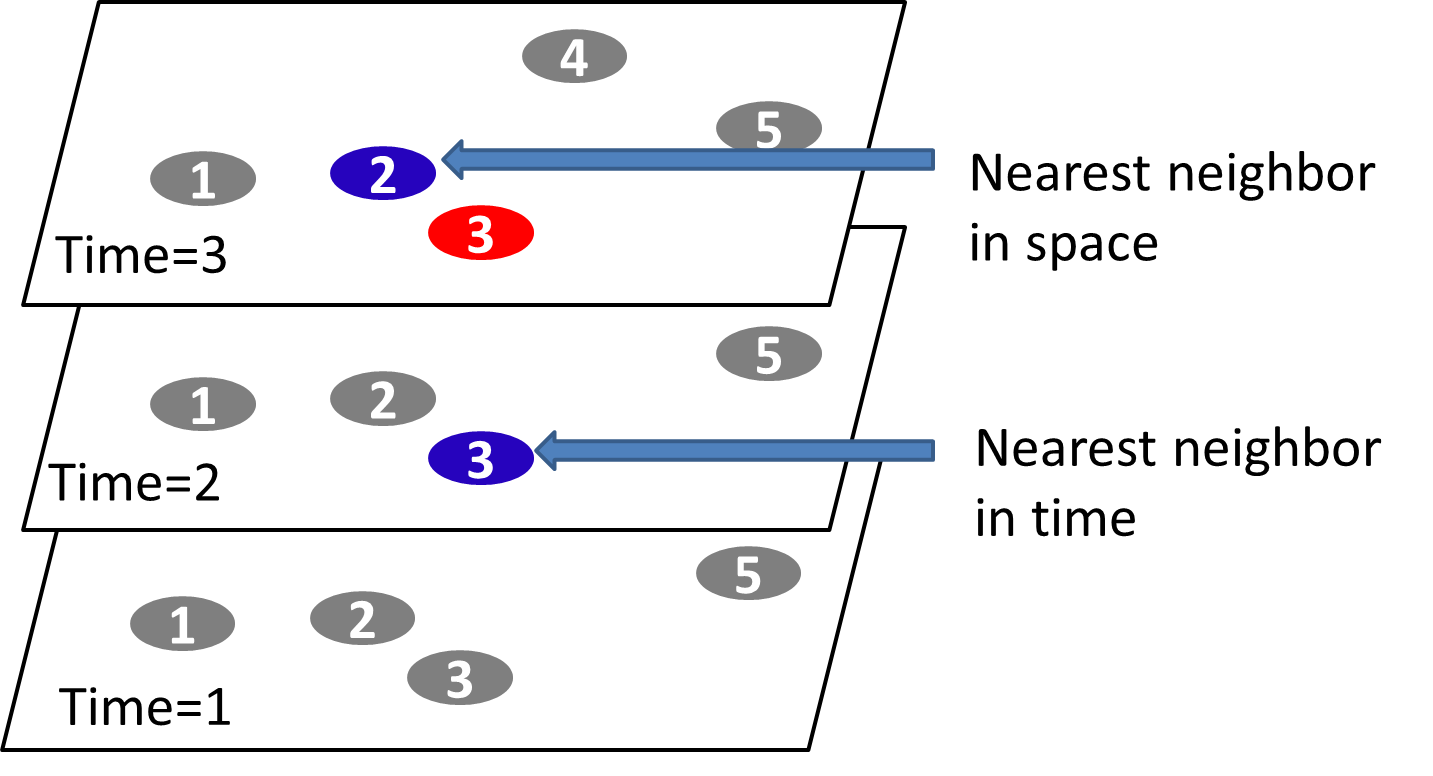
\includegraphics[scale=0.3]{../figures/stnn.png}
	\begin{itemize}
		\myitem For spatial NNGP, neighbors were chosen based on Euclidean distances
		\myitem No universal definition of distance in a space-time domain
		%\myitem Same problem in spatial data with incompatible dimensions
	\end{itemize}
\end{frame}

\begin{frame}{Adaptive neighbor sets}
%	\centering 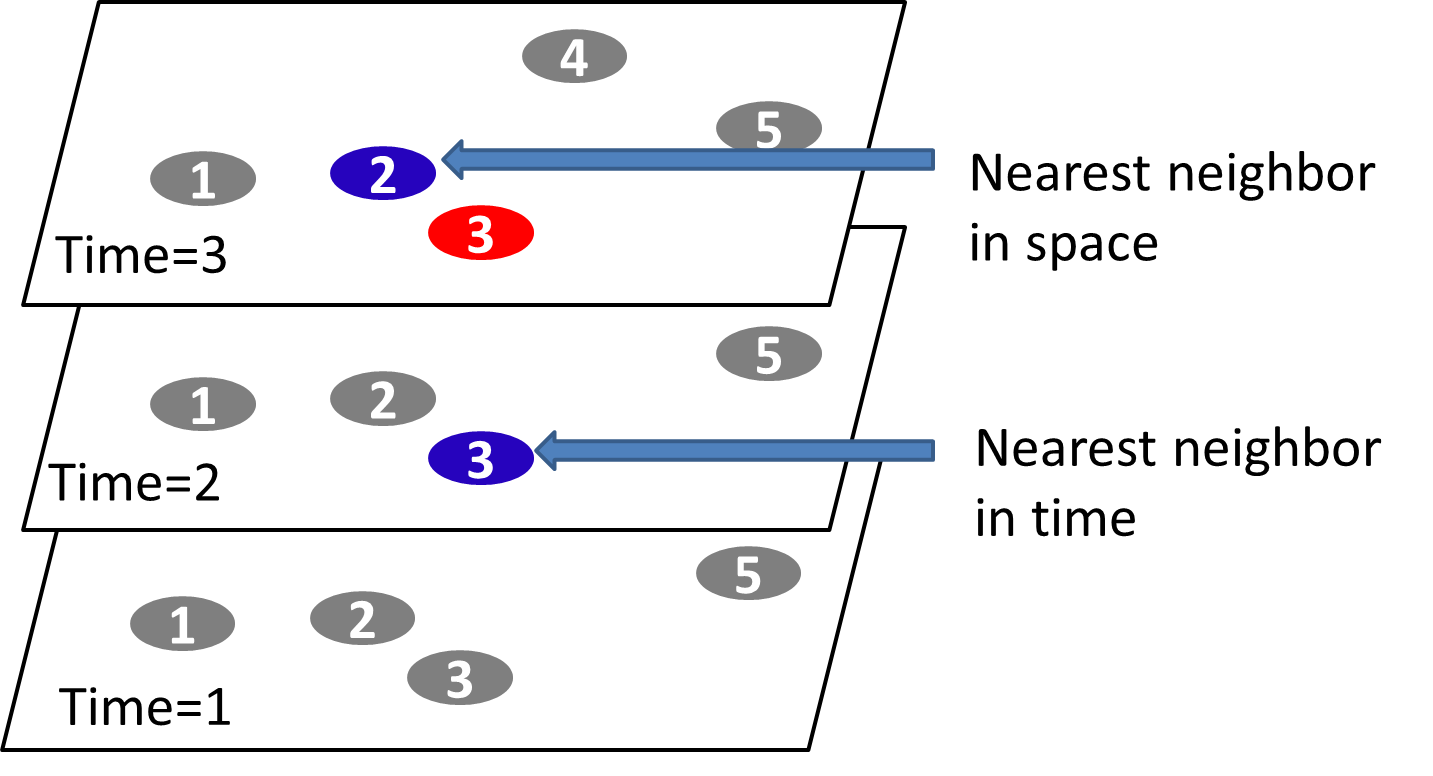
\includegraphics[scale=0.3]{../figures/stnn.png}
	%\end{frame}
	
	%\begin{frame}{Neighbors in Space and Time}
	
	\begin{itemize}
		\myitem Most popular spatial covariance functions decrease with increasing distance between locations
		\myitem So for spatial data, choosing nearest neighbors make sense as they correspond to locations with highest correlations with the given location
		%\myitem Spatio-temporal covariance functions decay both with the spatial and temporal lag
		\pause
		\myitem For spatio-temporal data, if $\theta$ is known, we can use $C(\cdot , \cdot \given \theta )$ directly to choose the neighbor sets
		\myitem Construct \red{adaptive neighbor sets} $N_\theta(s_i,t_j)$ using $m$-`nearest neighbors' based on $C_{\theta}(\cdot , \cdot)$ -- %inside $H_{ij}$ 
		\alert{Dynamic NNGP}
		%\myitem Neighbor sets now depend on $\theta$
		%\myitem Construct a spatio-temporal NNGP --- Dynamic NNGP
	\end{itemize}
	
\end{frame}
\begin{frame}{Computational Roadblock}
\begin{itemize}
\myitem Neighbor sets now \red{depend on $\theta$}
\begin{figure}[t]
%\vskip -2cm 
\begin{center}
\hskip -5mm 
\subfloat[$N_{\theta_1}(s,t)$]{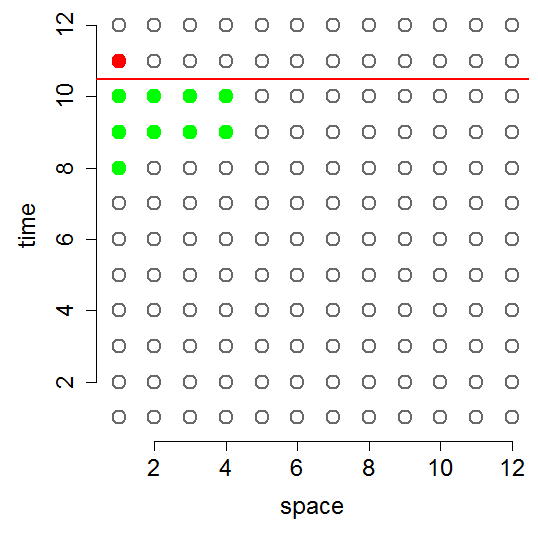
\includegraphics[width=3cm]{../figures/nei1.png}} %\hskip -3mm
\subfloat[$N_{\theta_2}(s,t)$]{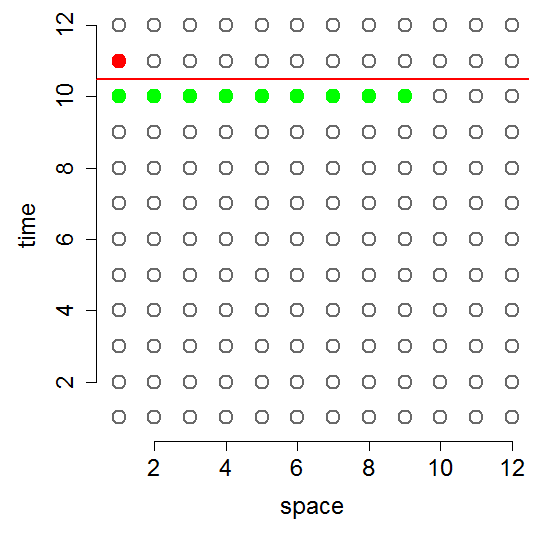
\includegraphics[width=3cm]{../figures/nei2.png}}
\end{center}
\caption{Adaptive neighbor sets (green) of the red point for different choices of $\theta$}
\end{figure}
\item Need to be \red{updated} after every update of $\theta$ in the MCMC
\item Computationally inefficient: 
\begin{itemize}
\item Need to calculate pairwise correlations for all locations
\item \textcolor{red}{$O(n^2)$} flops
\end{itemize}
\end{itemize}
\end{frame}


\begin{frame}{Updating Neighbor Sets}
\metroset{block=fill}
\begin{alertblock}{Eligible sets}
For every $(s_i,t_j)$ in $R$ one can construct an \alert{\em `eligible set'} $E(s_i,t_j)$ such that 
\begin{enumerate}[(a)]
\item $E(s_i,t_j)$ does not depend on $\theta$
\item For every value of $\theta$, $N_\theta(s_i,t_j) \in E(s_i,t_j)$
\item For $m \sim 20$, $|E(s_i,t_j)| \sim 4m$ for every $i,j$
\end{enumerate}
\end{alertblock}
\only<1>{
\begin{figure}[t]
%\vskip -2cm 
\begin{center}
\hskip -5mm \vskip -1.4cm
\subfloat[Not eligible]{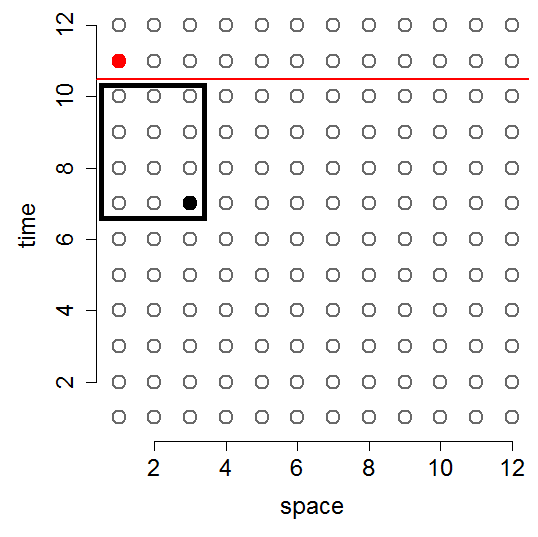
\includegraphics[width=3.5cm]{../figures/eliconstruct1.png}} %\hskip -3mm
\subfloat[Eligible]{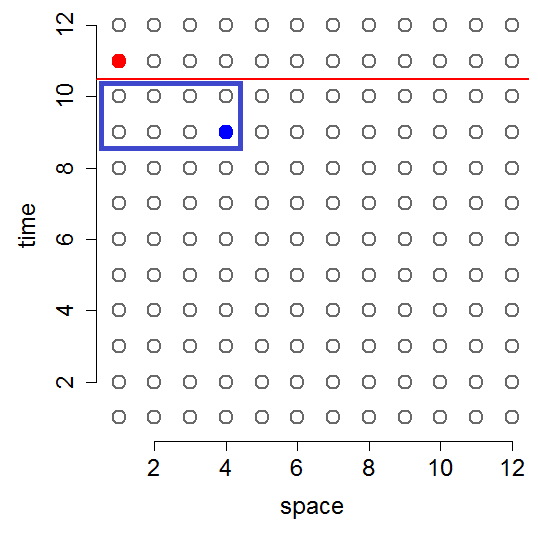
\includegraphics[width=3.5cm]{../figures/eliconstruct2.png}}
\subfloat[Eligible set ($m=9$)]{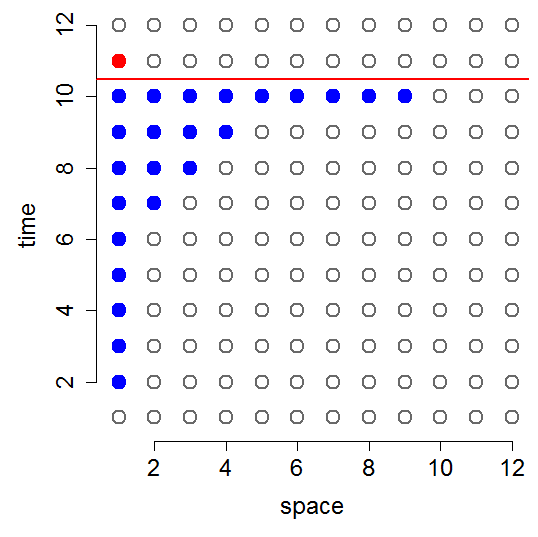
\includegraphics[width=3.5cm]{../figures/eli.png}} \hskip -3mm
\end{center}
\end{figure}
}
\only<2>{
\begin{figure}[t]
%\vskip -2cm 
\begin{center}
\hskip -5mm \vskip -1.4cm
\subfloat[$N_{\theta_1}(s,t)$]{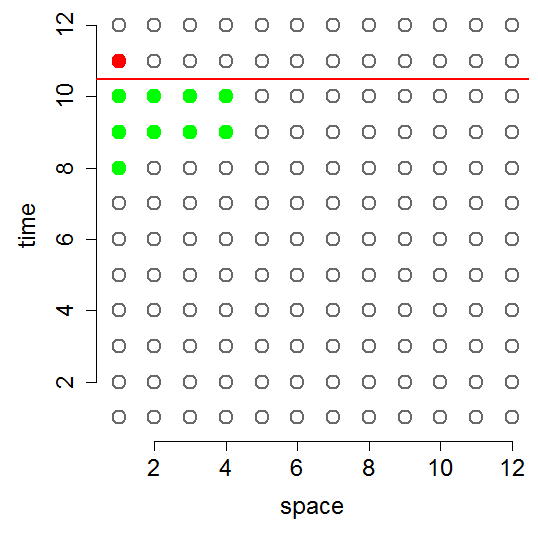
\includegraphics[width=3.5cm]{../figures/nei1.png}} %\hskip -3mm
\subfloat[$N_{\theta_2}(s,t)$]{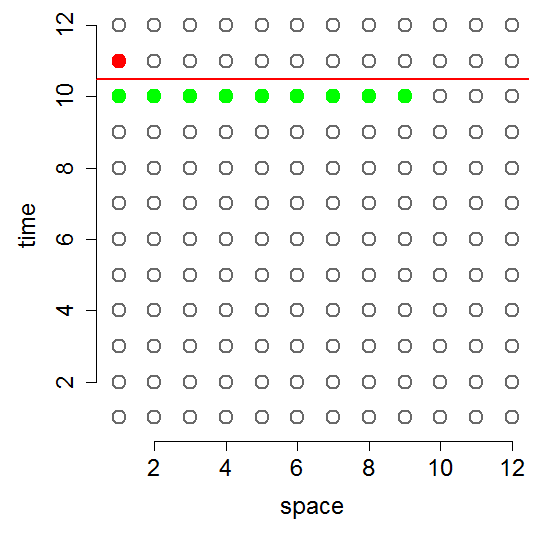
\includegraphics[width=3.5cm]{../figures/nei2.png}}
\subfloat[Eligible set ($m=9$)]{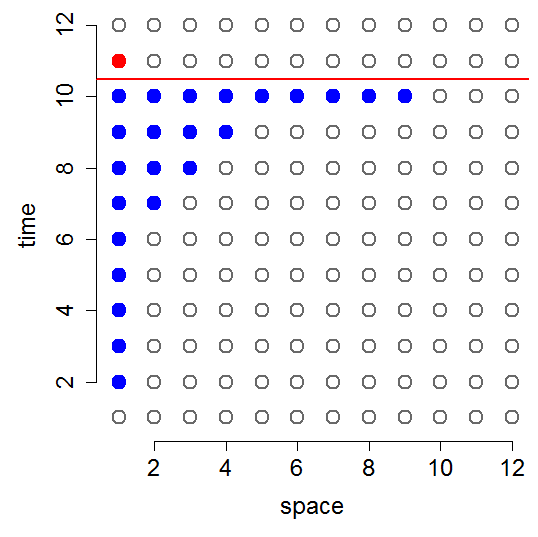
\includegraphics[width=3.5cm]{../figures/eli.png}} \hskip -3mm
\end{center}
\caption{Blue points denote the eligible set of the black point, it contains the neighbor sets (green) for all parameter values} 
\end{figure}
}
\only<3>{\begin{itemize}
\item \vskip -3mm $E(s_i,t_j)$ needs to be \red{constructed only once}
\myitem For every update of $\theta$, search for $N_\theta(s_i,t_j)$ only in $E(s_i,t_j)$
\myitem Total computational cost for this step \textcolor{red}{$=O(4nm)$} i.e., at par with the rest of the sampler -- Datta et al., AOAS, (2016)
\end{itemize}}
\end{frame}

\begin{frame}{Simulation Experiments}
\begin{itemize}
\myitem $225$ locations on a $15\times15$ grid within a unit square
\myitem $20$ time steps within a $0$ to $1$ range
\myitem $y(s,t) =\beta_0 +\beta_1 x(s,t) + w(s,t)+ \eps(s,t)$ 
%\myitem $x(t,s)$ was generated from standard normal distribution
\myitem $w(\bs,t) \sim$  GP with non-separable space time covariance function \[
K(h; u) = \frac{\sigma^2}{(\phi_1|u|^2+1)}\exp\left(\frac{-\phi_2||h||}{(\phi_1|u|^2+1)^{0.5}}\right)
\]
\end{itemize}
\end{frame}

\begin{frame}{Model evaluation}
\begin{table}[]
\centering
%\caption{Univariate synthetic data analysis}
{\scriptsize
\begin{tabular}{cccc}
  \hline
                & DNNGP & Predictive Process &Full\\
                       &$m=25$            &64 knots          & Gaussian Process \\ 
  \hline
%  $G+P=D$\footnote{Gelfand and Ghosh, 1998} &690&\textcolor{red}{2947}&734\\
  DIC score &3866&\textcolor{red}{7012}&3988\\
  RMSPE  &0.53&\textcolor{red}{0.71}&0.53\\  \hline
  Run time (Hours) &\textcolor{blue}{8}&14&\textcolor{red}{127}\\
\hline
\end{tabular}
}
\end{table}

\begin{itemize}
%\item Parameter estimates for all models are similar
\item DNNGP performs at par with Full GP, PP performs worse
\item DNNGP yields huge computational gains
\end{itemize}
\end{frame}

\begin{frame}{European Particulate Matter Dataset}
\begin{itemize}
\item Particulate matter (PM)
\begin{itemize}
\item Environmental pollutant associated with increased human morbidity and mortality
\item PM$_{10}$ (PM with diameter $< 10 \mu m$)
\end{itemize}
\myitem EU countries face legal action if PM$_{10}$ \red{exceeds 50 $\mu g$ $m^{-3}$} for more than 35 days per year
\myitem Accurate high-resolution regional space-time PM maps required for monitoring \green{compliance}
\end{itemize}
\end{frame}


\begin{frame}{European PM$_{10}$ Dataset}
\begin{figure}[]
\begin{center}
\vskip-4mm{\subfloat[PM$_{10}$ levels in March, 2009]{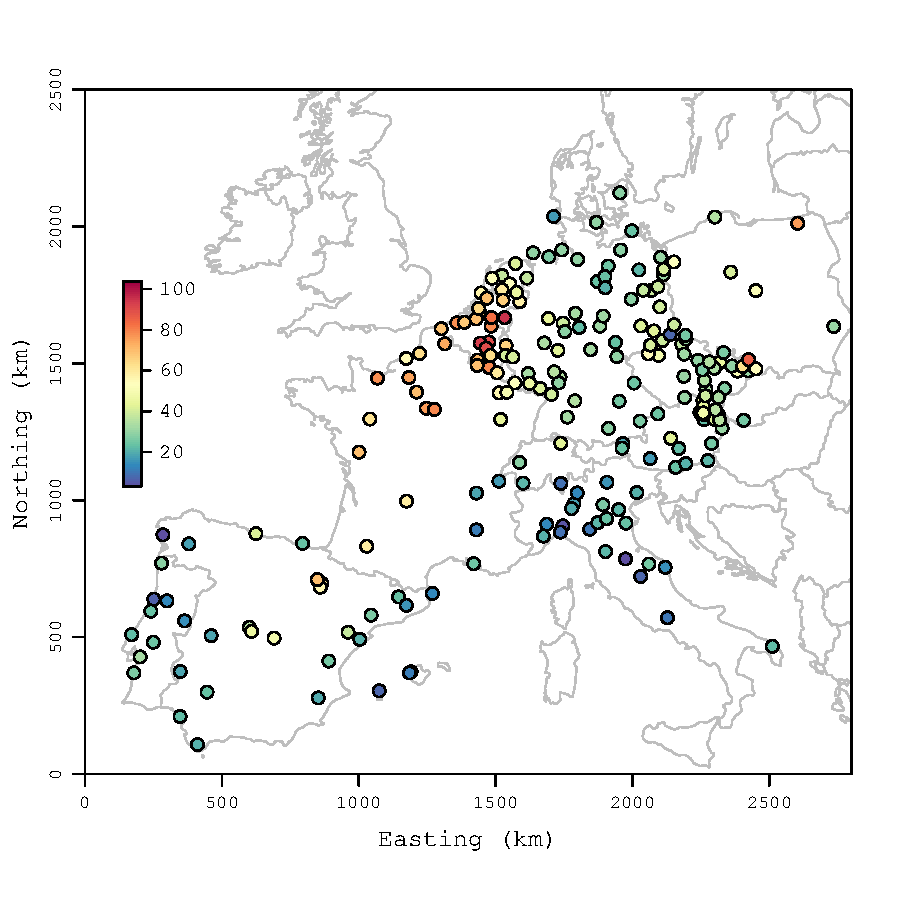
\includegraphics[width=5cm]{../figures/march-obs.pdf}\label{march-obs}}}
\subfloat[PM$_{10}$ levels in June, 2009]{{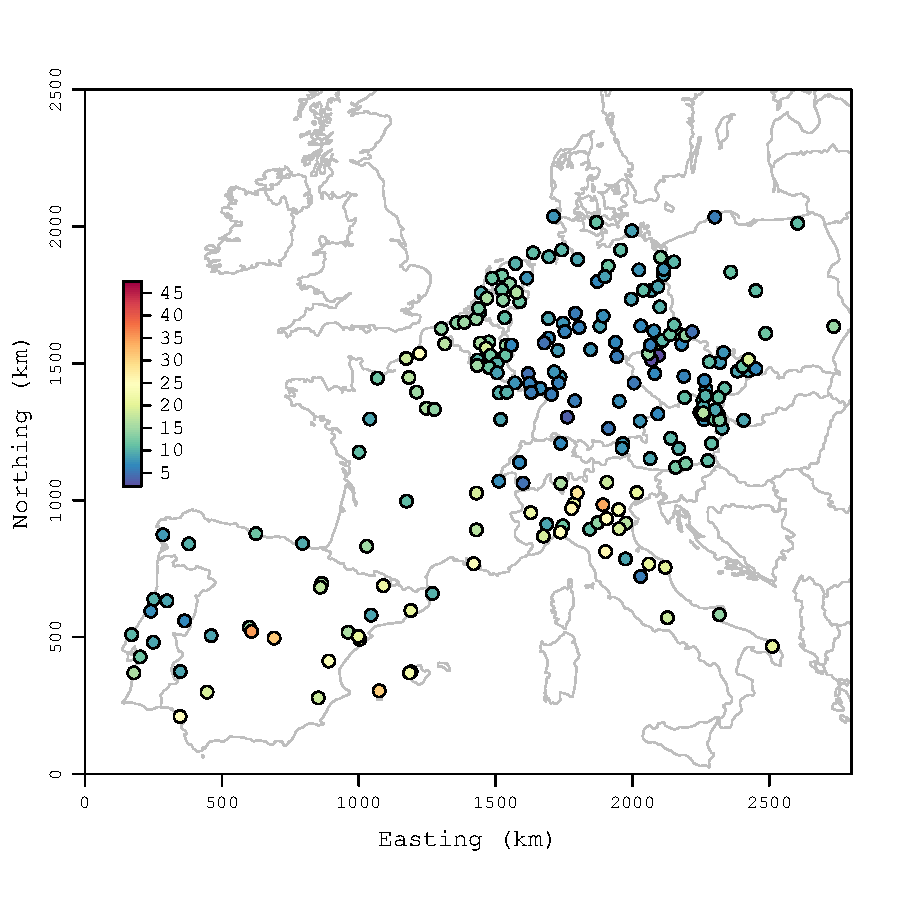
\includegraphics[width=5cm]{../figures/june-obs.pdf}\label{june-obs}}}
\end{center}
\end{figure}
\vspace{-0.5cm}
\begin{itemize}
\myitem Significant variation across space and time
\myitem Daily observations at $308$ stations for 2 years i.e., $n=308\times 730=$ \textcolor{red}{$224,840$}
\end{itemize}
\end{frame}

\begin{frame}{European PM$_{10}$ Dataset}
\begin{columns}[T] % align columns
\begin{column}{.48\textwidth}
\begin{figure}
\centering
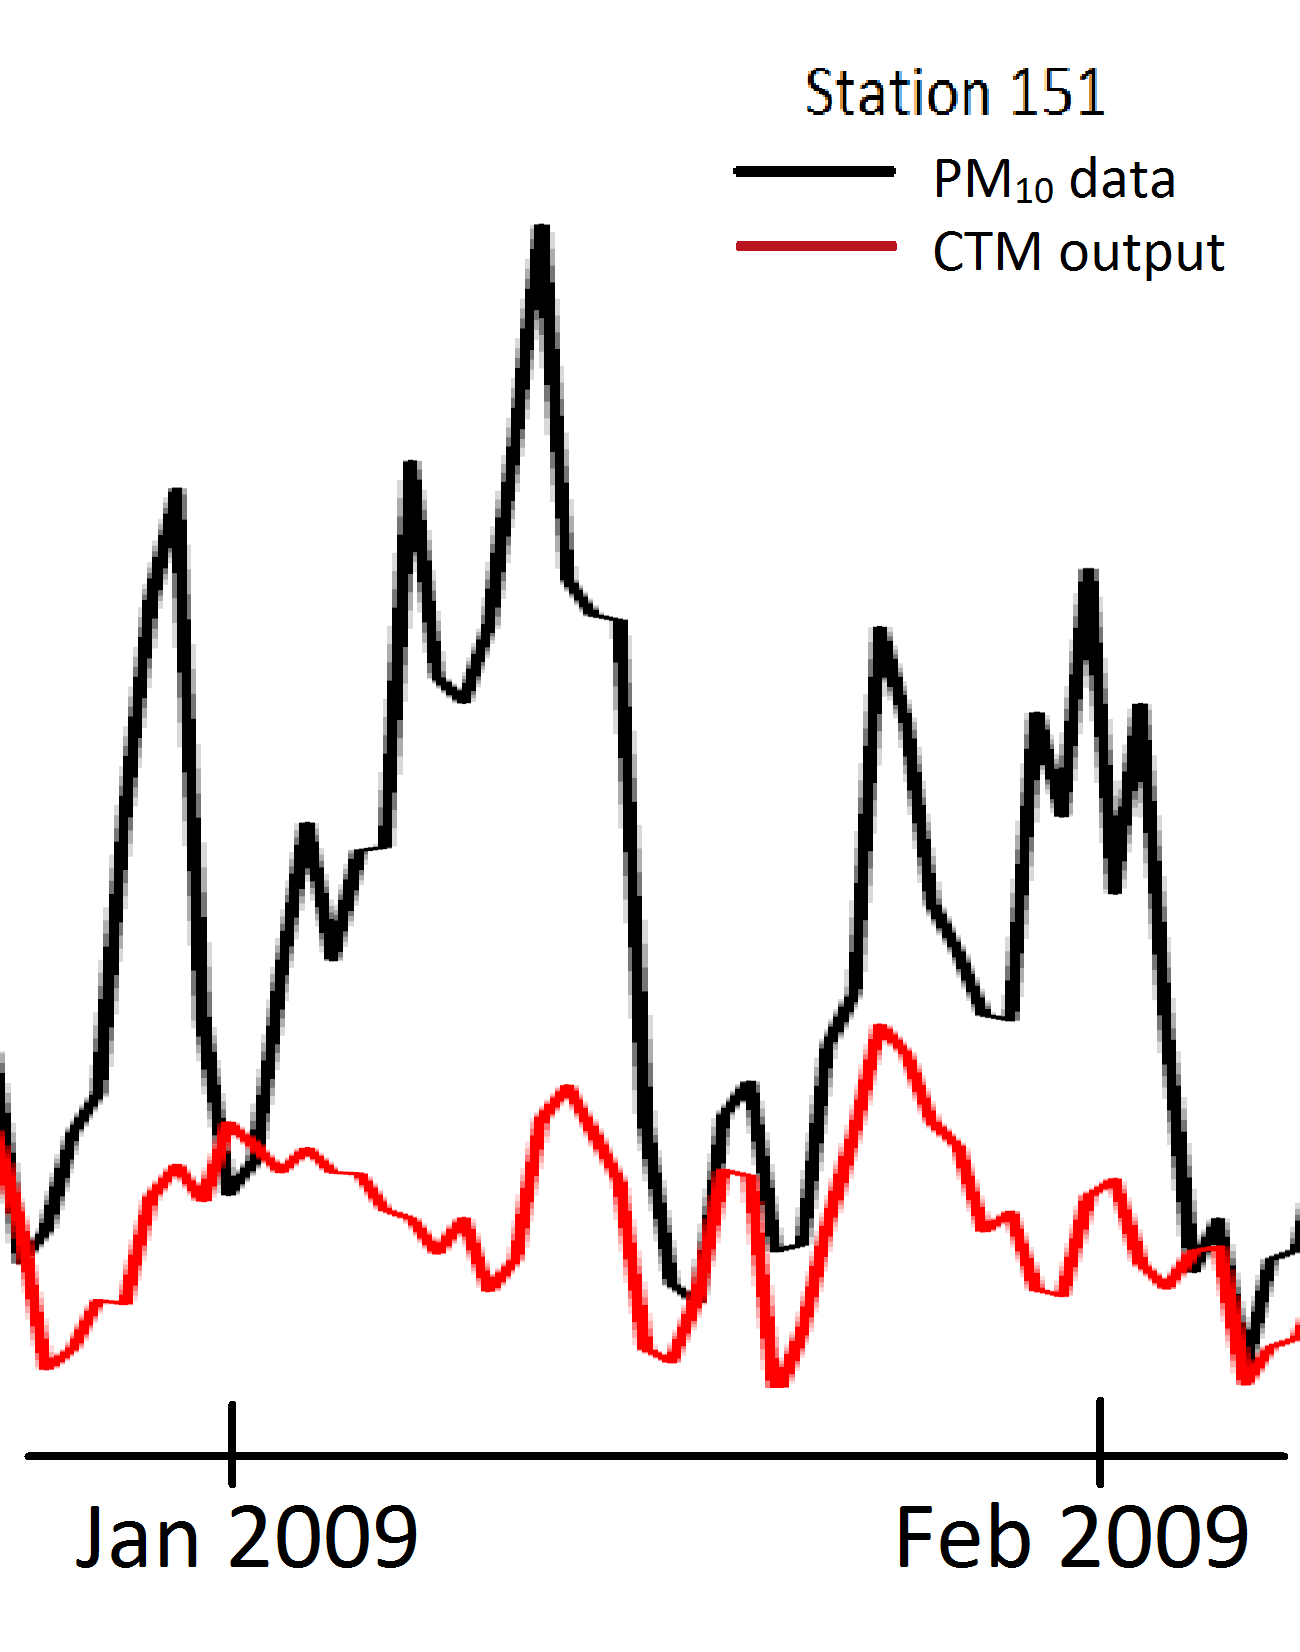
\includegraphics[scale=0.15]{../figures/ctmtest.png}
\end{figure}
\end{column}%
\hfill%
\begin{column}{.48\textwidth}
\vskip 0.5in
\begin{itemize}
\myitem Computer models like Chemistry Transport Model (CTM) consistently \red{underestimate} PM$_{10}$ levels
\myitem CTM outputs used as covariates to improve fits
$\log(PM_{10})(s,t) =\beta_0 +\beta_1 CTM(s,t) + \eps(s,t)$\end{itemize}
\end{column}%
\end{columns}
\end{frame}

\begin{frame}{European PM$_{10}$ data}
\begin{figure}[]
\begin{center}
\vskip-4mm{\subfloat[PM$_{10}$ levels in March, 2009]{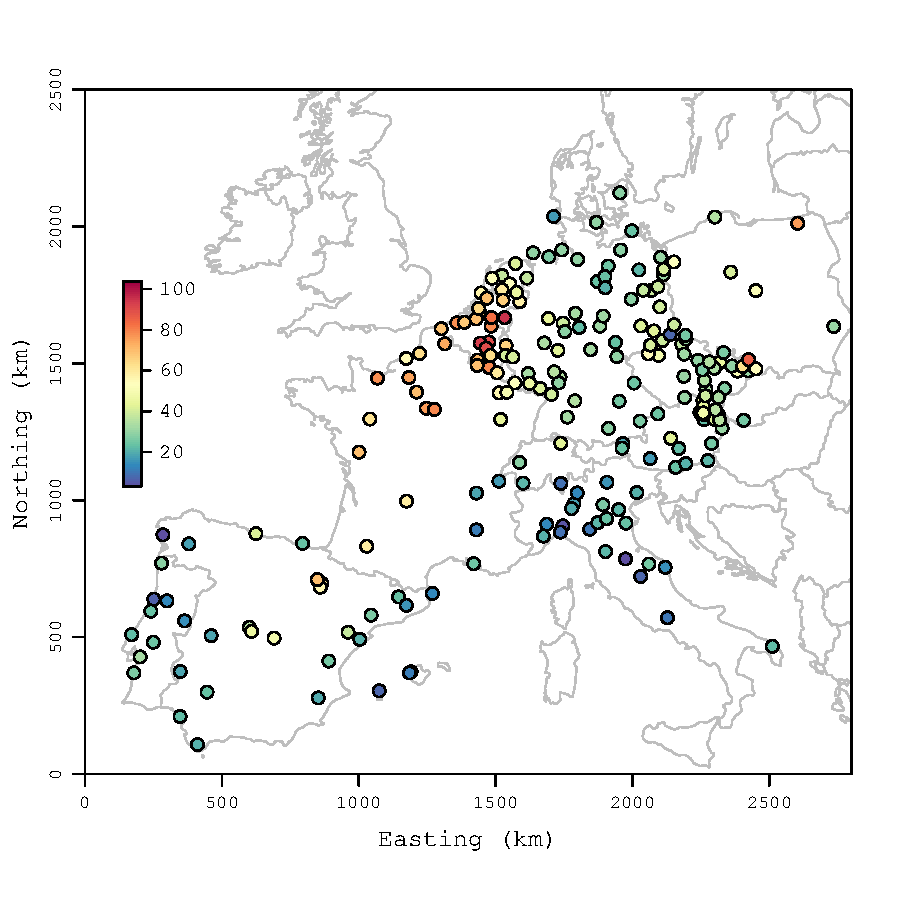
\includegraphics[width=5cm]{../figures/march-obs.pdf}\label{march-obs}}}
\subfloat[PM$_{10}$ levels in June, 2009]{{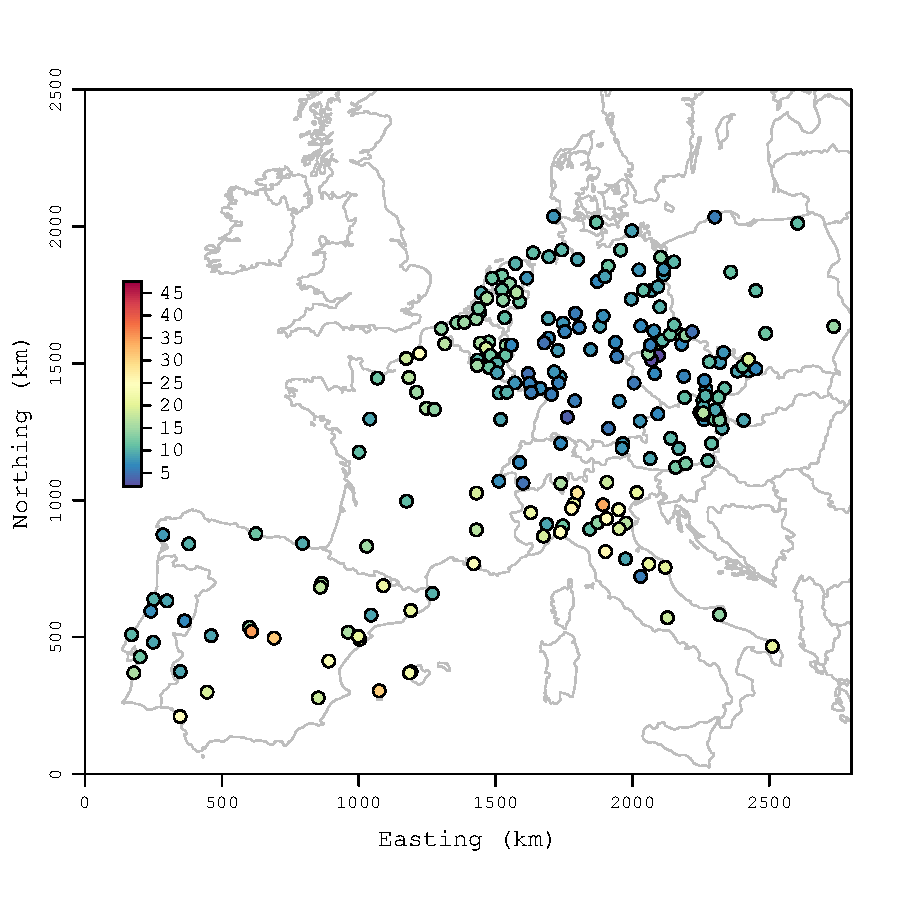
\includegraphics[width=5cm]{../figures/june-obs.pdf}\label{june-obs}}}
\end{center}
\end{figure}

\metroset{block=fill}\begin{block}{Model}
\begin{itemize}
\myitem $\log(PM_{10})(s,t) =\beta_0 +\beta_1 CTM(s,t) + w(s,t)+ \eps(s,t)$ 

\myitem $w(s,t) \sim \red{DNNGP}(0,\tkt)$
\end{itemize}
\end{block}
\end{frame}

\begin{frame}{European PM$_{10}$ Dataset}
\begin{columns}[T] % align columns
\begin{column}{.48\textwidth}
\begin{figure}
\centering
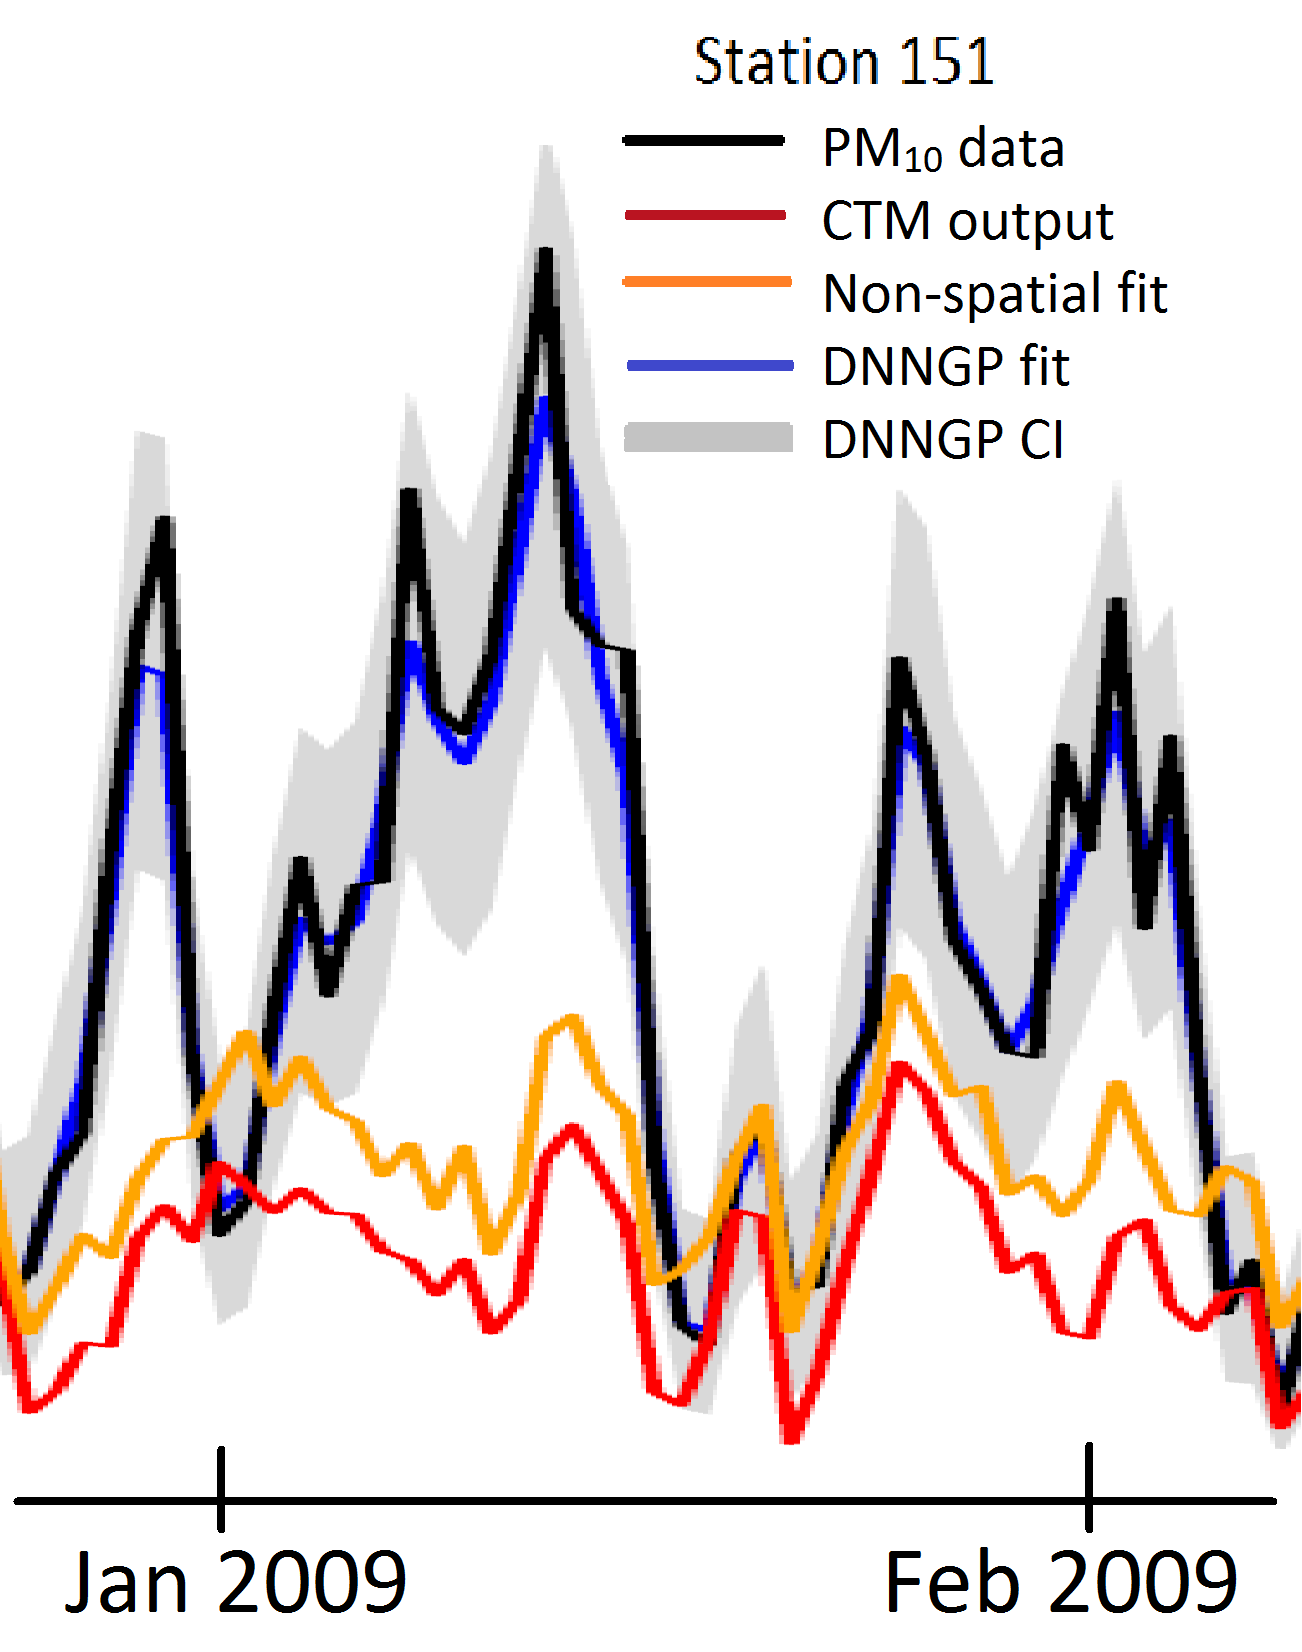
\includegraphics[scale=0.15]{../figures/pm10test.png}
\end{figure}
\end{column}%
\hfill%
\begin{column}{.48\textwidth}
\vskip 8mm
\begin{itemize}
\myitem Significantly improved fit
\vskip 5mm
\begin{tabular}{c|c|c}
& OLS & DNNGP \\ \hline 
RMSPE & 12.8 & 8.2 
\end{tabular}
\vskip 1cm 
\myitem Total time $24$ hrs
\end{itemize}

\end{column}%
\end{columns}
%\caption{Fitted and observed PM$_{10}$ for Station 23: PM10 observed (black), non space-time, regression (orange), CTM output (red), and m=20 DNNGP (blue) with associated 95\% CI band (gray). Prediction assessment holdout and actual missing observations are indicated with green and black points respectively. }
\end{frame}

\begin{frame}{European PM10 Dataset}
\begin{figure}[h!] 
\centerline{
\subfloat[m=10]{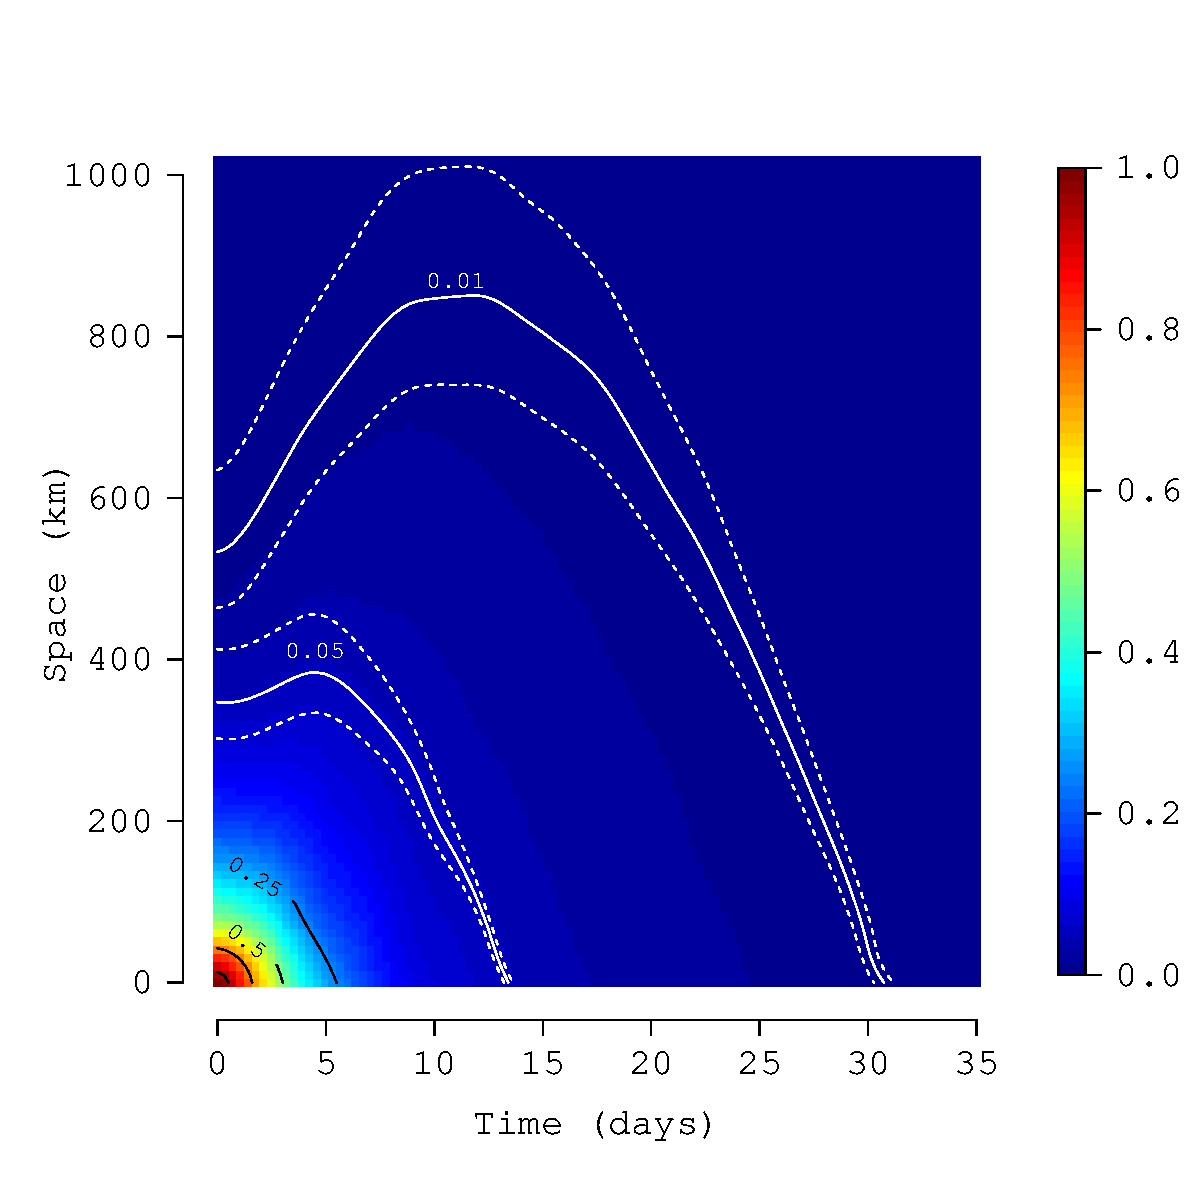
\includegraphics[trim={0 1cm 0 2cm},clip,width=1.8in]{../figures/rho-m15.pdf}} 
\hfil
\subfloat[m=20]{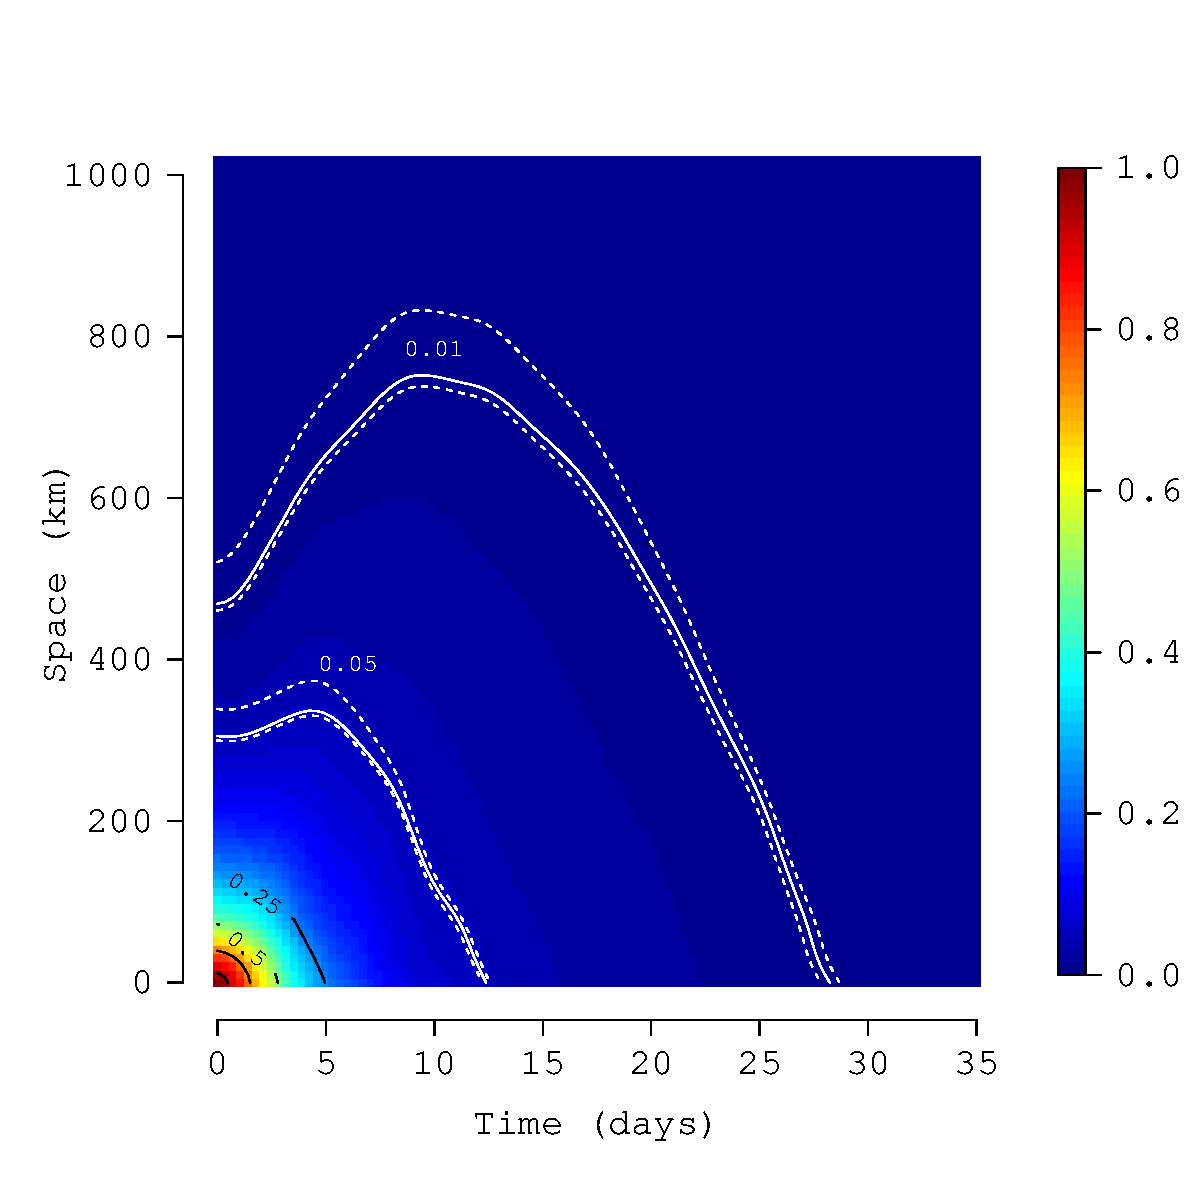
\includegraphics[trim={0 1cm 0 2cm},clip,width=1.8in]{../figures/rho-m20.pdf}} 
}
\caption{Space-time correlation posterior distribution median surfaces. Median (white lines) and associated 95\% credible intervals (dotted white lines) for correlations of 0.05 and 0.01.}\label{sptime-eff-rng}
\begin{itemize}
	\item Posterior distribution of the space-time covariance parameters provides insight into the residual spatio-temporal structure
	%\item This can be used to understand PM$_10$ better and improve the CTM
\end{itemize}
\end{figure}
\end{frame}


\begin{frame}{European PM$_{10}$ Dataset}
\begin{figure}
\begin{center}
\only<1>{\vskip-8mm\subfloat[$\widehat{\mbox{PM}_{10}}$ for 04.03.2009]{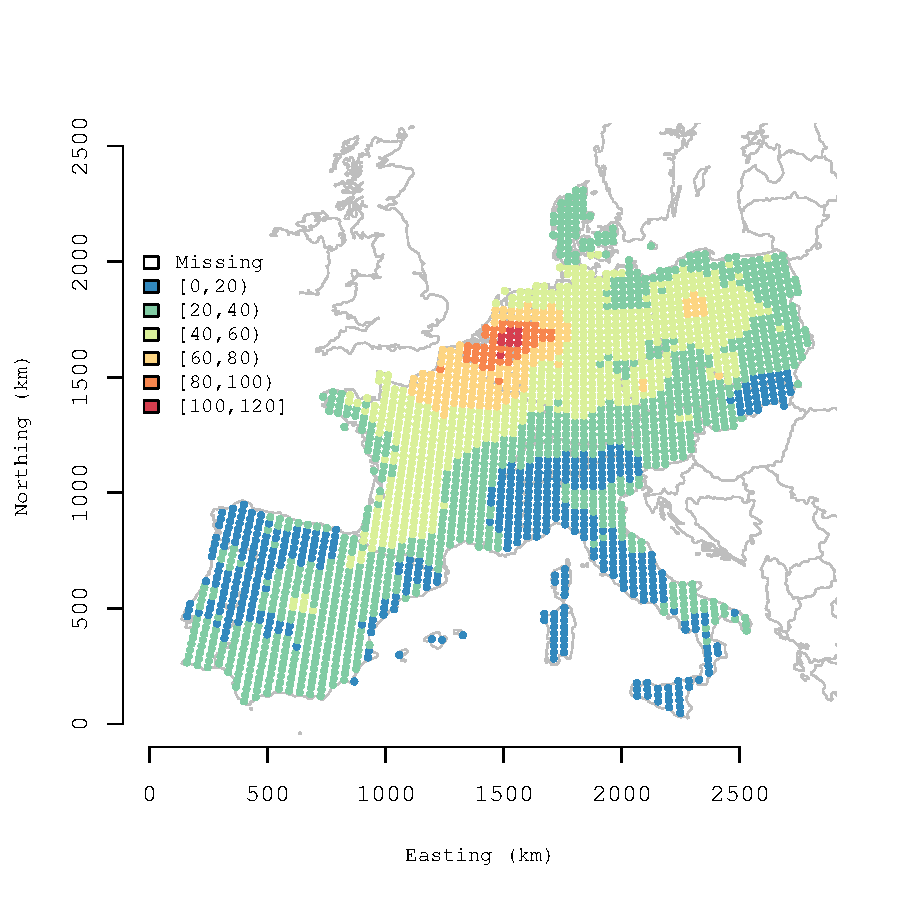
\includegraphics[width=5cm,trim={2.5cm 3cm 1cm 2cm},clip]{../figures/2009-4-3-ctm-grid-pred-mu.pdf}}
\subfloat[$Pr(\widehat{\mbox{PM}_{10}} > 50 \mu g m^{-3})$]{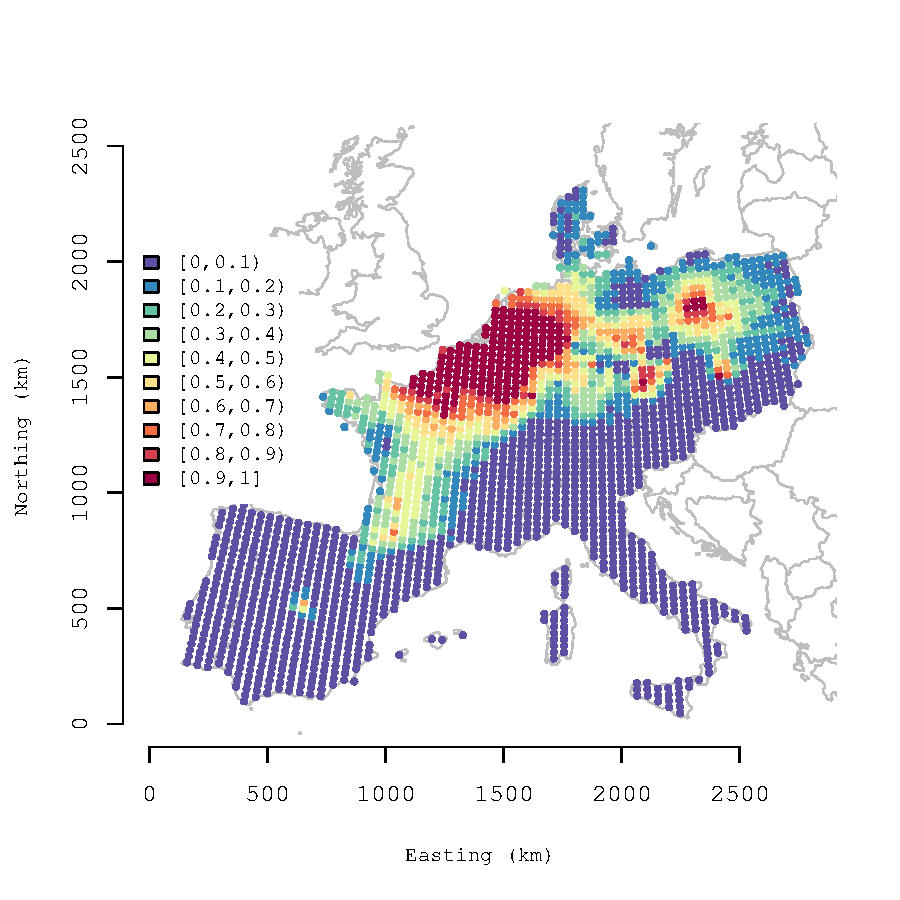
\includegraphics[width=5cm,trim={2.5cm 3cm 1cm 2cm},clip]{../figures/2009-4-3-ctm-grid-pred-prob-over-50.pdf}}}

\only<2>{\vskip-8mm\subfloat[$\widehat{\mbox{PM}_{10}}$ for 04.05.2009]{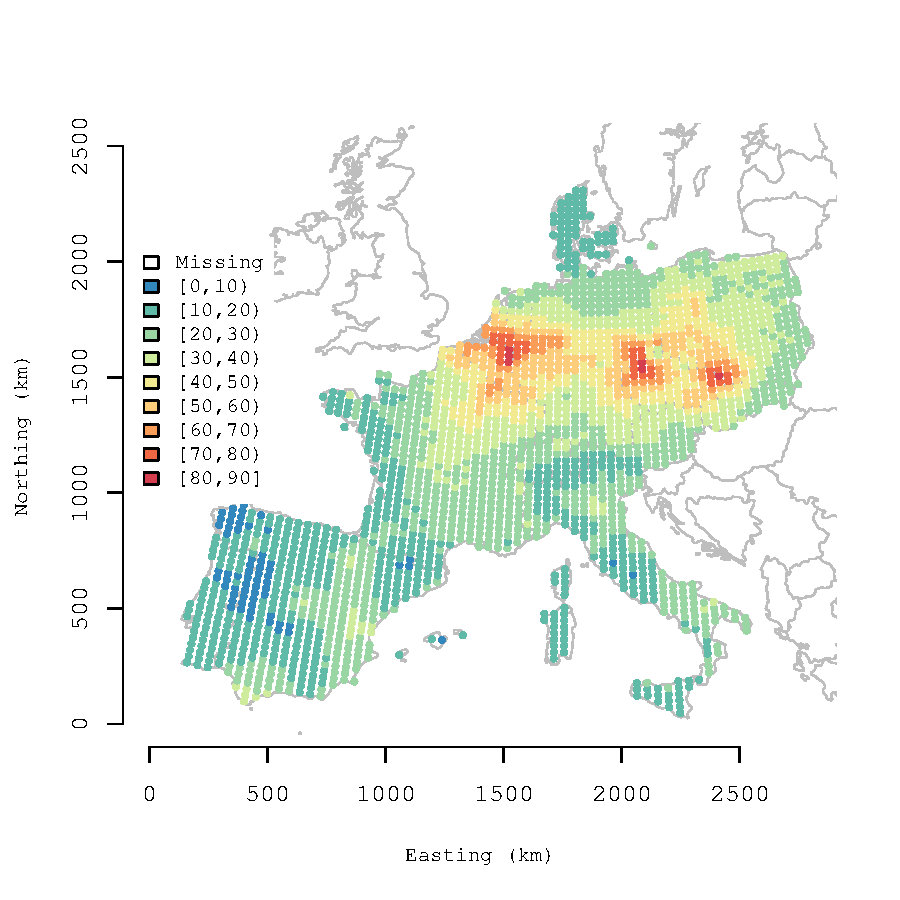
\includegraphics[width=5cm,trim={2.5cm 3cm 1cm 2cm},clip]{../figures/2009-4-5-ctm-grid-pred-mu.pdf}}
\subfloat[$Pr(\widehat{\mbox{PM}_{10}} > 50 \mu g m^{-3})$]{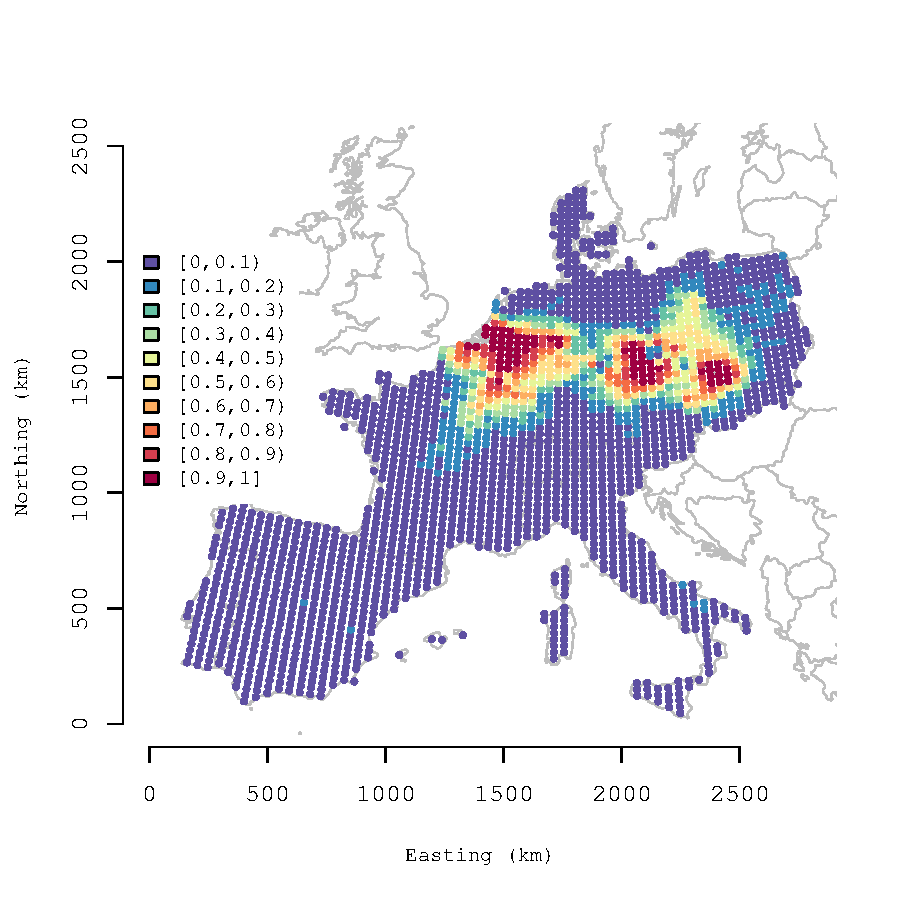
\includegraphics[width=5cm,trim={2.5cm 3cm 1cm 2cm},clip]{../figures/2009-4-5-ctm-grid-pred-prob-over-50.pdf}}}
\end{center}
%\vspace{-0.5cm}\caption{Predicted PM$_{10}$ and probability of exceeding 50 $\mu g$ $m^{-3}$ for two different dates}
\caption{Posterior predictve maps of PM$_{10}$ and of probability that PM$_{10}$ exceeds the legal threshold}
\end{figure}
\end{frame}

\begin{frame}{Summary}
\begin{itemize}
\item Spatio-temporal regression models -- discrete time continuous space, separable and non-separable continuous space time models
\item \red{Dynamic NNGP} for non-separable models for large spatio-temporal data
\item Neighbor sets chosen based on strength of spatio-temporal covariance
\item Fast algorithm to update the neighbor sets 
\item Retains all computational advantages of spatial NNGP: total requirements is \red{$O(n)$}
\item Performs at par with the original non-separable GP
\item Proper Gaussian process: Fully Bayesian inference, produces a variety of \blue{space-time forecast maps} at arbitrary resolution
\end{itemize}
\end{frame}

\end{document}
